\documentclass[tikz,border=2pt]{standalone}
% HiPaG architecture pipeline (vector, grayscale, print-safe).
% Build: latexmk -pdf architecture.tex   (from paper/figs)
\usepackage{times} % serif, matches sn-jnl body
\usepackage{amsmath} % \text in math mode
\usetikzlibrary{arrows.meta,positioning,fit,backgrounds}

\begin{document}
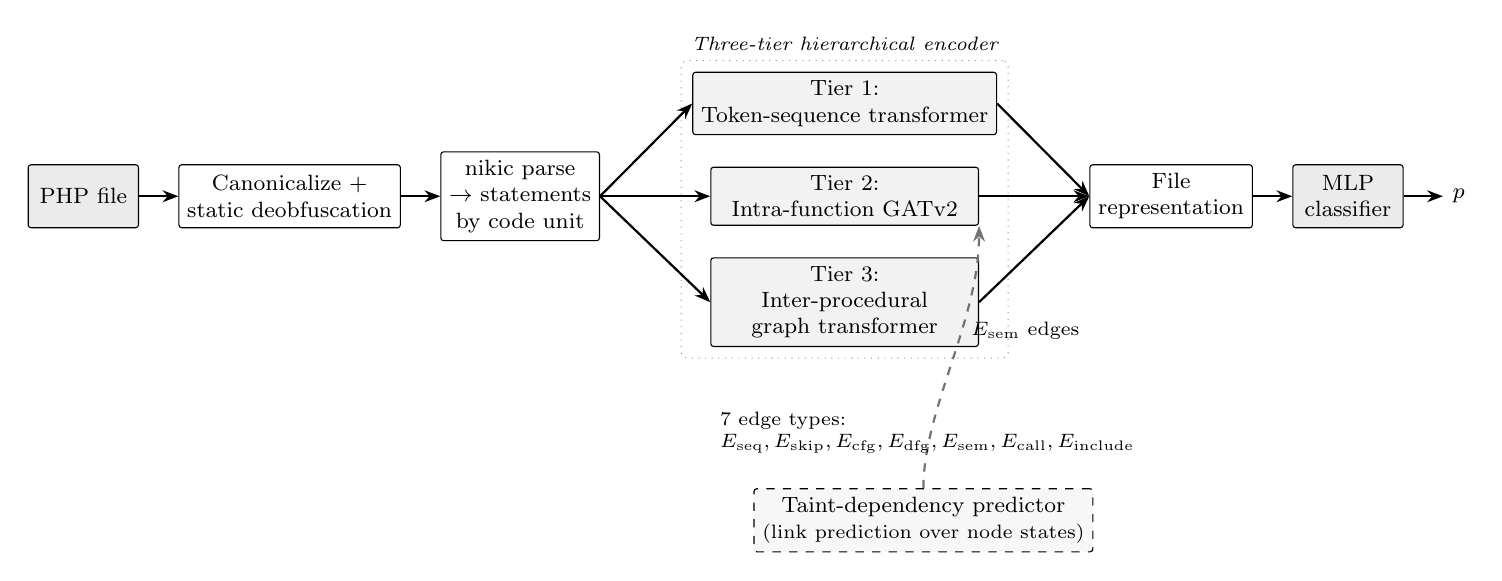
\begin{tikzpicture}[
    font=\footnotesize,
    >={Stealth[length=2mm]},
    node distance=5mm,
    box/.style={draw=black, rounded corners=1pt, align=center,
                inner sep=3pt, minimum height=8mm, fill=white},
    stage/.style={box, minimum width=20mm},
    tier/.style={box, fill=black!5, minimum width=34mm, minimum height=7mm},
    aux/.style={box, dashed, fill=black!3, align=center},
    io/.style={box, fill=black!8, minimum width=14mm},
    arr/.style={->, thick, draw=black},
    arrd/.style={->, thick, dashed, draw=black!55},
  ]

  % --- front of pipeline (left to right) ---
  \node[io]    (php)   {PHP file};
  \node[stage, right=of php]  (canon) {Canonicalize +\\static deobfuscation};
  \node[stage, right=of canon] (parse) {nikic parse\\$\rightarrow$ statements\\by code unit};

  % --- three stacked encoder tiers ---
  \node[tier, right=14mm of parse] (t2) {Tier 2:\\Intra-function GATv2};
  \node[tier, above=4mm of t2]     (t1) {Tier 1:\\Token-sequence transformer};
  \node[tier, below=4mm of t2]     (t3) {Tier 3:\\Inter-procedural\\graph transformer};

  % group label for the encoder stack
  \begin{scope}[on background layer]
    \node[draw=black!40, dotted, rounded corners=2pt,
          fit=(t1)(t2)(t3), inner sep=4pt] (stack) {};
  \end{scope}
  \node[anchor=south, font=\scriptsize\itshape] at (stack.north)
       {Three-tier hierarchical encoder};

  % --- tail of pipeline ---
  \node[stage, right=14mm of t2] (fr) {File\\representation};
  \node[io, right=of fr]         (clf) {MLP\\classifier};
  \node[right=5mm of clf]        (p)   {$p$};

  % --- taint-dependency predictor (aux box feeding E_sem into tier 2) ---
  % shifted right so its arrow rises through clear space to tier 2
  \node[aux] (taint) at ([xshift=10mm,yshift=-22mm]t3.south)
       {Taint-dependency predictor\\\scriptsize(link prediction over node states)};

  % --- main flow arrows ---
  \draw[arr] (php)   -- (canon);
  \draw[arr] (canon) -- (parse);
  % parse fans into the three tiers
  \draw[arr] (parse.east) -- (t1.west);
  \draw[arr] (parse.east) -- (t2.west);
  \draw[arr] (parse.east) -- (t3.west);
  % tiers feed the file representation
  \draw[arr] (t1.east) -- (fr.west);
  \draw[arr] (t2.east) -- (fr.west);
  \draw[arr] (t3.east) -- (fr.west);
  \draw[arr] (fr)  -- (clf);
  \draw[arr] (clf) -- (p);

  % taint predictor supplies E_sem edges to tier 2
  \draw[arrd] (taint.north) .. controls +(0,10mm) and +(0,-12mm) .. (t2.south east)
       node[pos=0.62, right, font=\scriptsize] {$E_{\text{sem}}$ edges};

  % edge-type note, parked at the bottom-left clear of all boxes
  \node[anchor=north west, font=\scriptsize, text width=52mm]
       at ([yshift=-7mm]t3.south west)
       {7 edge types: $E_{\text{seq}}, E_{\text{skip}}, E_{\text{cfg}},
        E_{\text{dfg}}, E_{\text{sem}}, E_{\text{call}}, E_{\text{include}}$};

\end{tikzpicture}
\end{document}
